\section{Methods Evolution}
\label{sec:methods-evolution}

This section traces the project's method development chronologically. Four generations brought us from a single-pipeline numeric baseline to the seven-pipeline panel that motivated the hybrid. The headline observation at the end of this section---that no single pipeline dominates and the dominant pipelines are Pareto-incomparable---is what made the cascade necessary.

\subsection{Generation 1 (V1, early May 2026): numeric and text baselines}

The first complete system used three pipelines:

\begin{itemize}
\item \textbf{\hgb{} (Histogram Gradient Boosting)} on the 94 derived numeric features (logs, traces, metrics, k8s, plus delta-from-baseline and moving-average columns). Trained with sklearn defaults (\texttt{max\_iter}=300, \texttt{learning\_rate}=0.05, \texttt{max\_depth}=8, \texttt{l2\_regularization}=0.1, \texttt{random\_state}=42).
\item \textbf{BM25 over V1 humanized Jira corpus} as a retrieval baseline. The V1 corpus was customer-service-voice ($\sim$800 characters per ticket), used as a starting point.
\item \textbf{Log-template anomaly} (logsense, a Drain-lite template miner) over per-window log lines. Useful as a third channel.
\end{itemize}

V1 results were mixed. \hgb{} hit PR-AUC = 0.77 on the first version of the test split---a strong triage baseline. BM25 retrieval was much weaker; the V1 corpus's customer-service phrasing rarely matched the engineering vocabulary in the window evidence text. We concluded the corpus realism, not the retriever, was the bottleneck.

A second observation from V1: the original train/test split was \emph{family-orphan-leaky}. The test set contained scenario families that did not appear in train. A model that had never seen \texttt{cart-redis} training data was being tested on \texttt{cart-redis} windows; unsurprisingly it failed. We rebuilt the split to be family-stratified (every family in train and test, different runs), producing the v2 in-distribution split (4{,}701 / 1{,}011 / 1{,}008). All subsequent results are on this split.

\subsection{Generation 2 (V2 SOTA, mid-May 2026): the multi-channel skill chain}

The V2 corpus redesign---engineer-voice tickets with embedded code blocks averaging $\sim$2400 characters and 90.2\% \texttt{description\_code} coverage---was the structural change that unblocked retrieval. With realistic prose, lexical similarity between window evidence and past tickets became meaningful.

The V2 SOTA pipeline (\texttt{memorygraph\_v2\_sota\_nw080}) is a deterministic skill chain that runs the following steps per window:

\begin{enumerate}
\item \textbf{entity\_extract}: parse \texttt{(service, component, error\_class, severity)} from the window evidence using rule-based extractors.
\item \textbf{component\_filter}: pre-filter the memory corpus to tickets sharing at least one extracted entity.
\item \textbf{lexical\_similarity (BM25)}: BM25 retrieval over the filtered memory pool.
\item \textbf{log\_signature\_similarity}: the ``Move A'' characteristic-log-line extractor produces one or two signature log lines per side; signatures are matched directly.
\item \textbf{cross\_encoder\_rerank}: an off-the-shelf \texttt{cross-encoder/ms-marco-MiniLM-L-6-v2} joint-scores the top-20 candidates; the final similarity is a $0.6 \cdot \text{crossenc} + 0.4 \cdot \text{biencoder}$ blend.
\item \textbf{graph\_score}: a bridge-weighted score over an entity-graph (rule-extracted) elevates tickets connected to the same components.
\item \textbf{numeric\_blend}: a separate \hgb{} head on the 94 numeric features.
\item \textbf{triage\_decide}: final triage probability $= 0.80 \cdot \text{numeric} + 0.20 \cdot \text{max\_combined\_sim}$.
\end{enumerate}

V2 SOTA achieved Hit@5 = 0.789 on the v2 in-distribution split (locked as the v2a-resplit baseline)---a step-change improvement over V1.

\begin{figure}[h]
\centering
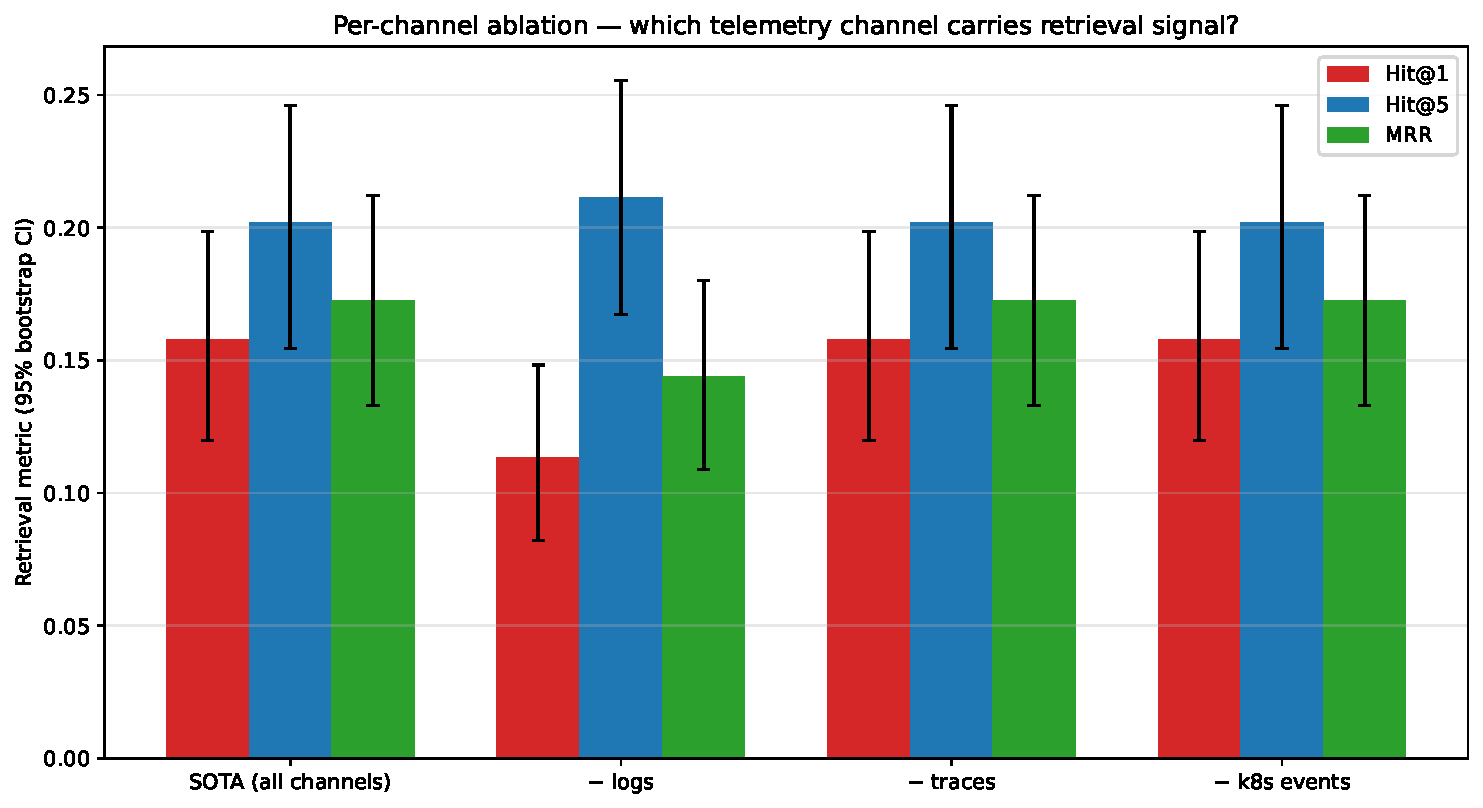
\includegraphics[width=0.85\linewidth]{figures/channel_ablation.pdf}
\caption{Per-channel ablation of the V2 SOTA pipeline. Each row drops one telemetry channel (logs, traces, or k8s events) from \emph{both} the window evidence and the memory ticket text, then measures the Hit@5 delta. Every channel contributes measurably; logs carry the largest contribution, followed by traces, then k8s events. The redundancy is intentional: a system that relies on a single channel would degrade silently when that channel's quality drops in production.}
\label{fig:channel-ablation}
\end{figure}

\subsection{Generation 3 (V2-advanced, late May 2026): bringing in LLMs and the graph}

Five orthogonal proposals were developed in parallel during this generation.

\textbf{Proposal A (resplit).} Repackaged the V2 SOTA on the in-distribution split. Locked as the baseline for everything that follows.

\textbf{Proposal B (\logseq{}).} A small transformer over raw log sequences, trained for 5 epochs in $\sim$14 minutes. Modest standalone performance (Hit@5 = 0.531) but uniquely good on specific families---it hit Hit@5 = 1.000 on \texttt{productcatalog-outage}. The signal it carries is \emph{complementary} to what BM25 captures.

\textbf{Proposal C (\hrrf{}).} A Reciprocal Rank Fusion of three sub-retrievers internally: BM25, a dense bi-encoder, and a rule-extracted graph score. The internal RRF uses $k = 60$ (the original RRF paper constant), top-10 from each. Standalone Hit@5 = 0.798---the first single pipeline to materially beat V2 SOTA on Hit@5.

\textbf{Proposal D (\kgret{} and LLM-graph hybrid).} We hypothesized that LLM-extracted graph entities would be more precise than rule-extracted ones. We ran Qwen 3.6 35B-A3B (via LM Studio) over all 347 humanized tickets with a strict JSON schema, extracting structured information per ticket: affected services, components, error classes, root cause, fix, symptoms. The output populated a Neo4j knowledge graph with 347 incident nodes, 12 service nodes, 27 component nodes, 803 symptom nodes, 343 root-cause nodes, 313 fix nodes, and 15 error-class nodes, connected via \texttt{Incident-AFFECTS-Service}, \texttt{Incident-HAS\_SYMPTOM-Symptom}, etc.

We ran the same skill chain as \hrrf{} but with the LLM-extracted graph in place of the rule-extracted one (denoted \hrrf{}-LLM). \emph{Counter-intuitively, the LLM graph produced a precision/recall trade-off}: Hit@1 went up +230\% relative against the rule graph (0.078 $\to$ 0.396), but Hit@5 went \emph{down} 39\% relative (0.555 $\to$ 0.337). We named this the ``RRF density paradox''---the LLM graph has high-precision but sparse signal, so fusion-based pipelines that depend on dense top-10 lists are starved.

\textbf{Proposal E (\agent{}).} We wrapped the LLM in a three-stage agent:

\begin{enumerate}
\item \textbf{Hypothesize} (thinking=OFF, $\sim$1 sec): given the window evidence, output a structured guess at the root cause.
\item \textbf{Retrieve} (no LLM call): use the L2 cascade to fetch the top-5 candidates.
\item \textbf{Verify} (thinking=ON, $\sim$25--30 sec): given the hypothesis + the top-5, output \texttt{\{best\_idx: int 0--4 or null, confidence: float 0--1, is\_novel: bool, reasoning: string\}}. If no candidate matches the hypothesis, \texttt{is\_novel = true}.
\end{enumerate}

Phase E pilots on 200 random windows found two things. (i) The agent's standalone retrieval Hit@5 was \emph{worse} than \hrrf{} (0.436 vs 0.789); the verify stage's stringent matching was too narrow. (ii) But the agent's novelty flag was extremely precise (94\%), and the free signal ``\texttt{max\_retrieval\_conf < 0.5}'' was independently precise at 96\%. We had two complementary novelty signals that, OR-ed, lifted recall from 7\% to 13\% at preserved precision.

\subsection{The Pareto-incomparable observation}

Table~\ref{tab:pareto-observation} reports each pipeline's headline standalone numbers on the v2 in-distribution split.

\begin{table}[h]
\centering
\caption{Each pipeline is dominant on one axis and dominated on others. \textbf{Bold} = best in column. The cascade exists because no single row is best everywhere.}
\label{tab:pareto-observation}
\small
\begin{tabular}{lrrrrr}
\toprule
Pipeline & Hit@1 & Hit@5 & MRR & PR-AUC strict & Novel detect? \\
\midrule
\hgb{} & --- & --- & --- & \textbf{0.9998} & no \\
\bienc{} & \textbf{0.695} & 0.789 & \textbf{0.729} & 0.287 & no \\
\hrrf{} rule & 0.583 & \textbf{0.798} & 0.669 & 0.236 & no \\
\hrrf{} LLM & 0.432 & 0.667 & 0.517 & 0.292 & no \\
\logseq{} & 0.483 & 0.531 & 0.498 & 0.313 & no \\
\kgret{} & 0.079 & 0.556 & 0.228 & --- & no \\
\agent{} (n=350) & 0.386 & 0.436 & 0.405 & 0.243 & \textbf{yes (94\% prec)} \\
\bottomrule
\end{tabular}
\end{table}

Every column has a different winner. \hgb{} owns triage but cannot retrieve. \bienc{} owns Hit@1 but loses Hit@5 to \hrrf{} rule. \hrrf{} LLM is precision-heavy and loses overall. \agent{} is the only novelty detector and is the worst retriever. No row Pareto-dominates any other row.

\subsection{Why this motivates a cascade rather than a bigger single model}

Two paths forward existed:

\begin{enumerate}
\item Build a bigger single model (a large transformer over evidence + memory + numeric features) and hope it learns the union of the per-pipeline signals.
\item Build a cascade that explicitly composes the per-pipeline signals.
\end{enumerate}

We rejected (1) for two reasons. First, the bottleneck inputs are heterogeneous (94-D numeric vectors, $\sim$2400-character text, log sequences, Neo4j graph queries). A single architecture that consumes all of them well is a research project of its own. Second, the signal from \hgb{} on numerics is \emph{already saturating} on this dataset (PR-AUC = 0.9998); a bigger model cannot beat 0.9998 by more than 0.0002. The marginal value of replacing \hgb{} with a transformer is negligible.

We chose (2). The cascade is interpretable, each layer optimizes one sub-task, and per-layer ablations can be run cleanly. The next section specifies the design.
